\documentclass{../template/texnote}

\title{\textbf{Probabilities in Machine Learning}}[author={Linn Abraham}]

\begin{document}
    \maketitle \currentdoc{note}
    %<*note>


\section{Introduction}

The concepts of randomness and probability are interlinked and at the same time quite important for a fruitful understanding of Machine Learning (ML).
You are bound to encounter them on your journey of being a researcher in ML, if you have not already. 
However if you think you understand both these concepts at least at the level of a definition, think again.
The field of probability for one, becomes more complicated the further you try to understand it. It can also be counter-intuitive at times. 
You might be surprised to find that there is no straight forward answer to the question of what is meant by ``probabilities".
There are in fact entire schools of thoughts when it comes to the interpretation of what are probabilities and how to use them. Two of the more popular ones are known as `Frequentism' and `Bayesianism'.


Christopher Bishop \nocite{bishop_pattern_2006} in his highly acclaimed textbook, mentions probability theory, decision theory and information theory as three important tools when it comes to learning machine learning.
This article motivates the need to pursue probability in machine learning by listing some common applications. Then it tries to give an overview of the difficulties in understanding probabilities by listing some of the different interpretation of probabilities. After that we introduce two concepts that are crucial to understanding probabilities - the concept of a probability distribution function and Bayes theorem which is one of the most important concepts in probability theory. 
The last two discussions are heavily inspired from the works of 3Blue1Brown. \nocite{3b1b}


% This article tries to explore some of the connections between probability theory and machine learning.
% A common encounter of probability for a machine learning practitioner is when they try to interpret the output of activation functions as a probability score.
% Elsewhere you might have come across terms such as "Bayesian Networks" or "Bayesian classifiers".
% Once you understand the connection between probability and machine learning such things might hopefully become clear to you.


\section{Use in Machine Learning}
Randomness and probabilistic methods come up a lot in machine learning.  Here are a few of the more common ones.
There are learning algorithms that make use of randomness and probability concepts such as the \textbf{Random Forest}, the \textbf{Naive Bayes Classifier} or even \textbf{Bayesian Neural Networks}.
\textbf{Genetic algorithms} are optimization algorithms inspired by randomness and natural selection.
\textbf{Gaussian processes} are a type of probabilistic model used for regression and classification tasks.
\textbf{Bootstrapping} is a resampling technique used in ensemble methods like bagging.
\textbf{Expectation Maximization} or EM is an optimization algorithm used in unsupervised learning especially in clustering and \textbf{Gaussian Mixture Models} (GMM).
\textbf{Dropout } is a common regularization technique used in neural networks that drops random neurons during the training process.


Randomness is also important during the training process for initialization of model weights, train-test splitting of datasets, used in optimization methods such as stochastic gradient descent and even in random search during hyper-parameter tuning.
Often in ML, we try to interpret the outputs of activation functions etc. as probabilities.
A related aspect is how we design or interpret the common evaluation metrics that comes up in discriminant models like sensitivity, specificity etc.
This is one area where we need to use concepts from probability such as Bayes theorem for properly understanding the results.
%We often need to invoke the concepts of probabilities when evaluating performance of a trained discriminant model in ML. %To understand similar to diagnosis test in medicine etc.



\section{Interpretations of probability}
\subsection{Two types of probabilities}
There are two ways in which probabilities are used, which may be called physical (objective or frequency) and evidential (Bayesian) probabilities.
Physical probabilities are associated with physical systems that are considered random in nature such as rolling dice or radioactive decay.
There are events associated with such systems that happen at a fixed rate or relative frequency.
Physical probabilities are invoked to explain such stable frequencies.
This is the kind of probability that most people are introduced to during their primary education.

The other kind of probability, evidential probability, can be considered as a degree of belief in a statement as supported by available evidence.
It can be associated to any statement, even one without any kind of randomness involved.
This is a kind of probability that is used very informally in daily life but has more importance in academia and research.
The following are the four main interpretations of probabilities.
\subsection{Classical Interpretation (A priori)}
This interpretation is attributed to Pierre-Simon Laplace who assumed by what has been called the ``principle of insufficient reason", that all possible outcomes of an event are equally likely if there are no reasons to assume otherwise.
Probability of an event is then the ratio of number of outcomes favourable to the event to the total number of outcomes possible.

\subsection{Empirical Interpretation (A posteriori)}
This interpretation is sometimes called Frequentist. However the term is also used to refer to ``physical probability" as a whole when contrasting it with Bayesian probabilities.
According to this, the probability of an event is the relative frequency of occurence after repeating the process for a large number of times under similar conditions.

\subsection{Subjective Interpretation}
As mentioned above probabilities can be used as a measure of the degree of belief of an individual who is assessing the uncertainty of a situation.

\subsection{Axiomatic Interpretation}

The mathematics of probability can be developed on an entirely axiomatic basis that is independent of any interpretation.

\section{Interpreting Probability Density Functions (PDF)}
Probability density functions are ubiquitous in statistics and probability theory. To motivate the need for such a function we need to shift our thinking from a discrete context to a continuous context.
When you consider experiments such as tossing a coin or rolling a dice etc. the outcomes you are interested in are often discrete.
Like for e.g., the probability of getting two heads when a coin is tossed 5 times.
However one can imagine a case where the outcomes can take any value in a continuous range.
In such a case no matter how small a value you assign to each of these outcomes, you would run into a problem. The sum of all these would add upto infinity.
This means that in such a scenario it no longer makes sense to talk about probabilities of individual values.
However if we consider a histogram where the height of the bins represent the probability, that the outcome is within a range given by the bin widths, then we no longer have a problem.
It is the area of each bin that gives the probability associated with that range.
When you have bins of smaller and smaller widths you have a more refined knowledge of the probabilities in each individual bin.
And you also end up with a smooth curve.
But what is the height of this curve that we have ended up with?
Since the width of a bin times the height is a probability, the quantitiy in the y-axis would have a dimension of probability over length.
Hence what he have can be called a probability density.
Since the probabilities are represented by areas of the individual rectangles, the total area under the curve adds upto 1. 

When trying to interpret the probability distribution function as mentioned you might run into a problem.
The probability of getting an exact value, which is the area of a very thin slice becomes zero by definition.
To understand what is happening here, note that, if in the discrete case the probability of the outcome falling in one out of a collection of values was just the sum of the individual probabilities. 
In the continuous case, the probability of your outcome taking a range of values is no longer the sum of individual probabilities.
Instead the probabilities associated with the ranges themselves are the fundamental primitive objects we are dealing with here.
In order to make more sense of this you might have to learn a bit of measure theory a branch of mathematics which provides the foundational framework for the rigorous mathematical development of probability theory.

\section{Bayes Theorem: Evidence should not determine beliefs but update them}
\subsection{When to use Bayes theorem}
One of the most important formulas in probability theory is the Bayes formula.
Before we try to understand what the formula is telling us let us see when it would be useful to actually apply the formula.
Suppose you are shown the following description of a person called Steve.
``Steve is very shy and withdrawn, invariably helpful but with very little interest in people or in the world of reality.
A meek and tidy soul, he has a need for order and structure, and a passion for detail.
If you are then asked the following question, ``Which of the following do you think more likely: "Steve is a librarian" or "Steve is a farmer" ? 
Which one might you choose?

This example is part of a study conducted by Psychologists David Kahneman and Amos Tversky.
Their study showed that most people go with the option of Steve being a librarian.
Although it is true that these traits align with the stereotypical view of a librarian than a farmer, the authors of the study show that it is irrational to come to that judgement.
Their point was that almost no one thought of using the information about the ratio of farmers to librarians in their judgements.
The question is not whether the partcipants had information about those statistics but whether they thought about estimating it?

\subsection{How to use Bayes theorem}
Let's say you did estimate the ratio of farmers to librarians and came up with the number 20:1. 
So let us start with a sample size of 210 people. Of which there are 200 farmers and 10 librarians.
Next you think about all the librarians you know and come to the estimate that 40 percent of all librarians fit the description and 10 percent of all farmers fit the same description. That is you are still saying that a librarian is 4 times more likely to fit the description than a farmer.
However if you now try to find out the probability that a random person who fits the description is a librarian. It is given by, 

$$\frac{\textrm{ 4 Librarians who fit the description}}{\textrm{ 4 
 Librarians + 20 Farmers who fit the description}}$$

 Which is only 16 percent. Whereas the probability that the random person would be a farmer would be 84 percent.
 The key takeaway here is that new evidence should not determine your beliefs in a vaccuum; it should update prior beliefs.

 So the way to understand such problem is start to with all possibilities (210).
 Then seeing evidence restricts the space of possibilities ( 4 + 20).

\subsection{Motivating the Bayes formula}
 How can we generalize from this example to reach a formula?
 The general scenarios is the following. You have some hypothesis (or model) like the hypothesis that ``Steve is a Librarian" or ``The coin is fair".
 You have some evidence (data or observation) like the description about Steve that you obtained.
 You are mostly interested in knowing the probability that your hypothesis is true given the evidence. This is what you computed quite easily in the example above. The probability that ``Steve is a Librarian'' given the description about Steve which we can now denote $P (H|E)$.

 How did we arrive at the numerator which was 4? By first calculating the probability that the hypothesis holds without considering any of the evidence. This is called the prior and denoted $P(H)$. In our case we calculated the prior by taking the ratio of all librarians to farmers which came to be $1/21$.  
 After that we used the proportion of librarians that fit the description.
 This is the probability of seeing the evidence given the hypothesis is true.
 That is, if it is given that Steve is a librarian, we then limit our space of possibilities to the space of all librarians and ask how likely it is for a random librarian to have this description.
 This is also called the likelihood and in our case it was $4/10$.
 Now by multiplying the total number of people times the prior times the likelihood we obtain the numerator.

 In the denominator we again have the same term. But also an additional term which contains the likelihood of observing the evidence if the hypothesis is not true, which in our case was $1/10$.
 Along with this we need to multiply the the prior corresponding to the case where our hypothesis is not true and the total number of people.
 So finally putting all these words into an equation we have, 
 $$ P(E|H) = \frac{P(H)P(E|H)}{P(H)P(E|H)+P(\neg H)P(E|\neg H)}$$
% \section{Why use Probabilities?}
% Why do we toss a coin
% You might already know that true randomness is quite rare.
% Processes such as tossing a coin or throwing a dice which we use as substitutes for a truly random process are in fact

% \begin{figure}[htpb]
%     %\centering
%     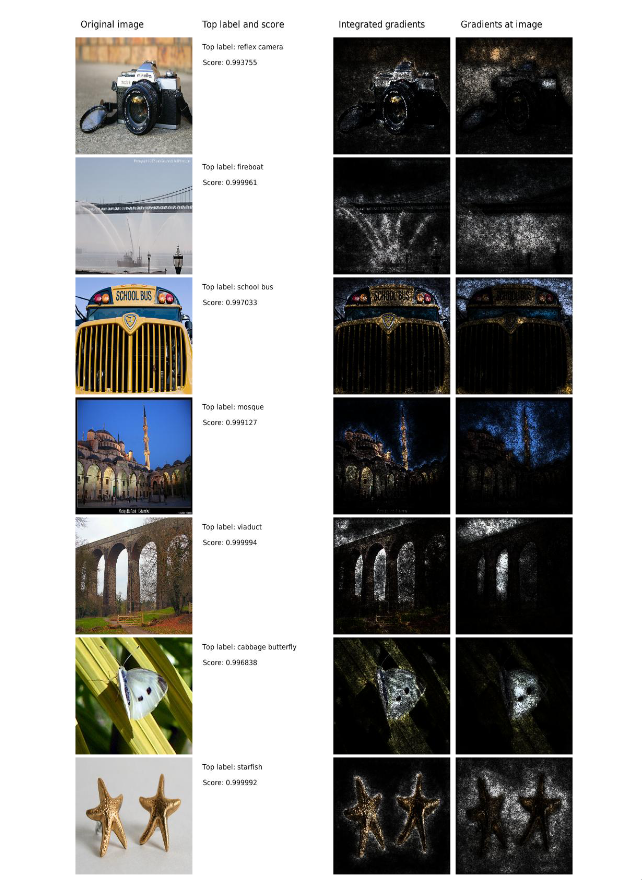
\includegraphics[width=\textwidth]{Linn/object_recognition.png}
%     \caption{\textbf{Comparing integrated gradients with gradients at the image.} Left-to-right: original input image, label and softmax score for the highest scoring class, visualization of integrated gradients, visualization of gradients*image. Notice that the visualizations obtained from integrated gradients are better at reflecting distinctive features of the image.}
%     \label{fig:object}
% \end{figure}

 \nocite{wikipedia}
 \nocite{3b1b_binomial}
 \nocite{3b1b_bayes}



\begin{thebibliography}{1}
\providecommand{\natexlab}[1]{#1}
\providecommand{\url}[1]{\texttt{#1}}
\expandafter\ifx\csname urlstyle\endcsname\relax
  \providecommand{\doi}[1]{doi: #1}\else
  \providecommand{\doi}{doi: \begingroup \urlstyle{rm}\Url}\fi

\bibitem[1]{bishop_pattern_2006}
Christopher~M. Bishop.
\newblock \emph{Pattern Recognition and Machine Learning}.
\newblock Information Science and Statistics. {Springer}, {New York}, 2006.
\newblock ISBN 978-0-387-31073-2.

\bibitem[2]{wikipedia}
{Probability interpretations}.
\newblock \url{https://en.wikipedia.org/wiki/Probability_interpretations}.

\bibitem[3]{3b1b}
{ 3blue1brown}.
\newblock \url{https://www.3blue1brown.com/}, {\natexlab{a}}.

\bibitem[4]{3b1b_binomial}
{ Binomial distributions | Probabilities of probabilities, part 1}.
\newblock \url{https://www.3blue1brown.com/lessons/binomial-distributions},
  {\natexlab{b}}.

\bibitem[5]{3b1b_bayes}
{ Bayes' theorem }.
\newblock \url{https://www.3blue1brown.com/lessons/bayes-theorem},
  {\natexlab{c}}.

\end{thebibliography}
\vspace{0.5cm}
\noindent\fbox{%
	\parbox{\textwidth}{%
		\textbf{About the Author}\vspace{0.2cm} \\
		\textbf{Linn Abraham} is a researcher in Physics, specializing in A.I. applications to astronomy. He iscurrently involved in the development of CNN based Computer Vision tools for classifications of astronomicalsources from PanSTARRS optical images. He has used data from a several large astronomical surveys includingSDSS, CRTS, ZTF and PanSTARRS for his research.
		
	}
}
    %</note>
    \printbibliography
\end{document}
